\section{Cloud Storage}


\subsection{Storage models}
    In cloud computing a massive amount of data needs to be handled. If years ago the most important service was the performance of cloud, nowadays it' reliability: data has to be stored and providers have to be able to make sure to not lose them.
    In order to provide reliability, different copies of the same data will be stored. The disadvantage is that maintaining consistency among multiple copies of data will require more software complexity.
    
    We define \textbf{storage model} the layout of a data structure in a physical storage.
    
    We define \textbf{data model} the set of logical aspects related to how to store data in a given space.
    
    Storage models must guarantee two features:
    \begin{itemize}
        \item Storage models must be \textbf{read/write coherent}: the result of a read operation of memory should be the same as the most recent write operation; in other words every operation of read operation needs to ensure that the previous write operation has been already completed.
        \item Storage models must respect the \textbf{before-or-after atomicity}: the result of an operation, from the point of view of the invoker, must be the same as if the actions occurred either completely before or completely after.
    \end{itemize}

    
\subsection{Block storage}
    Data are managed by means of blocks within sectors and tracks (this is very useful mostly for databases by DBMS).
    
    OpenStack Cinder is a Block Storage service for OpenStack. It's designed to present storage resources to end users, in particular it allows to interact with different row and not formatted hardware. 
    
    \begin{figure}[h!]
        \centering
        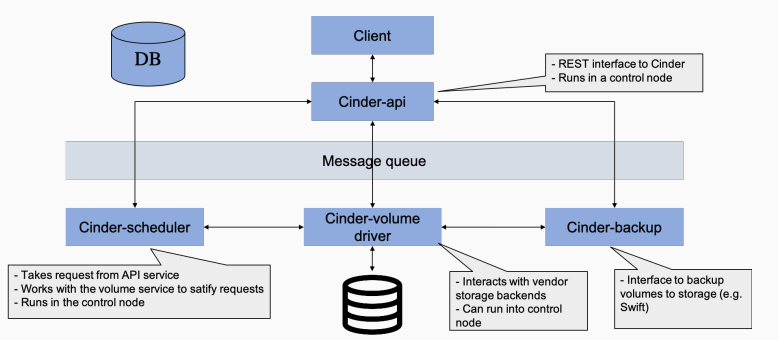
\includegraphics[scale=0.5]{images/Cinder architecture.png}
    \end{figure}
    
    The Cinder architecture is composed by:
    \begin{itemize}
        \item a volume driver that interacts with the vendor
        \item a scheduler that takes request from the API interface (like modifying a volume and snapshots).
        \item a backup that is an interface for backupping volumes.
    \end{itemize}


\subsection{Distributed file systems}
First of all, let's introduce some terms:
\begin{itemize}
    \item A \textbf{file} is a linear array of cells stored on a persistent storage device. From the point of view of applications it's viewed as a collection of logical record and is stored on a physical device as a set of physical records of size determined by the physical media.
    \item A \textbf{file pointer} is a cell used as a starting point for a read or write operation of a file.
\end{itemize}
Files could be organised as:
\begin{itemize}
    \item \textbf{Logical}: the organization reflects the data model. This is often the prospective the applications.
    \item \textbf{Physical}: the organization reflects the storage model and describes the manner the file is stored on a given storage media.
\end{itemize}

So a \textbf{file system} is a collection of directories (logical partition of the disk) and each one provides information about the organization of a set of files.
File system can be \textit{traditional} (like the Unix File System) or \textit{distributed} (like the Network File System ...).


\subsubsection{Unix File System}
The \textbf{Unix File System} (UFS) is based on three main points:
\begin{itemize}
    \item It's designed a \textit{layered} mode; this provides flexibility because:
    \begin{itemize}
        \item It allows UFS to separate the concerns for the physical structure (hardware) from the logical one (applications).
        \item \textit{inode} layer allows UFS to treat uniformly local and remote file access.
    \end{itemize}
    \item Its \textit{hierarchical} design supports scalability reflected by the file naming convention (like nested directory)
    \item \textit{Metadata} supports a systematic design philosophy of the file system and device-independence
    \begin{itemize}
        \item Metadata includes information like file owner, access rights, creation time etc. (information useful for managing files)
        \item \textit{inodes} contains information about individual files and directories
    \end{itemize}   
\end{itemize}   

\myparagraph{USF layering}
Lower layers are dedicated to the physical organization:
\begin{itemize}
    \item A \textit{Block layer} locates individual blocks on the physical device;
    \item A \textit{File layer} reflects organization of blocks into files;
    \item A \textit{Inode} layer provides metadata for the objects;
\end{itemize}

Upper layers are dedicated to the logical organization.

Than there's the File name layer (I/O layer) that mediates between machine and user oriented view of the FS. In particular it provides an API to allow communication between them.

\begin{figure}[h!]
    \centering
    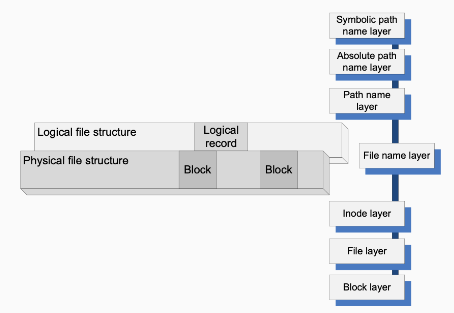
\includegraphics[scale=0.35]{images/UFSlayering.png}
    \caption{UFS layering}
    \label{fig:usfl}
\end{figure}


\subsubsection{Network File System}
The \textbf{network file system} (NFS) has been the first which was distributed. It has been created to have a sort of integration with the UFS.

Its design objectives are:
\begin{itemize}
    \item Provide the same semantics as a local UFS to ensure compatibility.
    \item Facilitate the integration into existing UFS.
    \item Support clients running on different operating system.
    \item Accept a modest performance degradation due to remote access.
\end{itemize}

NFS is based on the Client-Server paradigm: a Client runs on the local host while the server is at the site of the remote file system. Client and Server interact by means of Remote Procedure Calls (RPC).

In the NFS remote files are uniquely identified by a file handler (instead of a file descriptor).
\begin{figure}[h!]
    \centering
    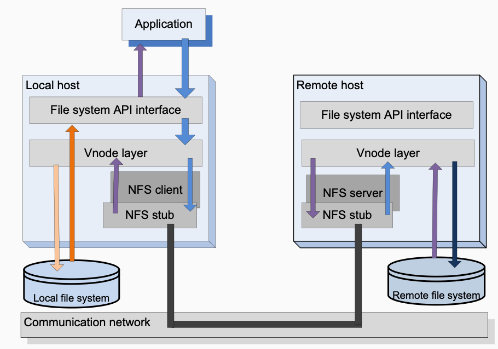
\includegraphics[scale=0.35]{images/NFS.png}
\end{figure}

On the local host and on the remote host there's a \textbf{vNODE layer} (corresponding of inode) that implements file operations in a uniform manner, regardless of whether the file is local or remote.

The mechanism of the client-server interaction in steps is:
\begin{itemize}
    \item An application request for a file;
    \item the vNODE layer of the remote host tries to understand if the file is local to the remote host or not;
    \item if it's not local, it will requests for it from the local host;
    \item the vNODE layer of the local host will receive the request for the file;
    \item if the file is present, the vNODE layer will sand it to the remote host;
    \item the vNODE of the remote host will direct the file to the remote file system.
\end{itemize}


\subsubsection{Design choices for distributed file system}
Distributed file systems have common features:
\begin{itemize}
    \item Common policy: conventionally when a file is close, the server should have the newest version on persistent storage;
    \item Policy to write a block:
    \begin{itemize}
        \item in \textit{write-backs} policy a block is first written to cache while the writing on the disk is delayed for a time (tens of seconds). This policy speeds-up the writing operation but it can cause data loss if the system fails;
        \item in \textit{write-through} policy a block is written to the disk as soon as it's available on the cache. This policy increase reliability but requires more time to complete the writing operation;
    \end{itemize}
    \item Concurrency:
    \begin{itemize}
        \item in \textit{sequential write-sharing} a file cannot be opened simultaneously for reading and writing operations by several clients (preferable). This policy is allowed by some unique access algorithms that can locks files;
        \item in \textit{Concurrent write-sharing} a file can be opened and modified by multiple clients (often not acceptable);
    \end{itemize}
    \item Parallel I/O executions: if allowed, it implies the execution of multiple input/output operations. To allow the parallel execution, the concurrency need to be handled in some way.
\end{itemize}


\subsection{General Parallel File System}
The \textbf{General Parallel File System} (GPFS) is the first file system invented. It's structured in some servers connected with LANS.

\begin{figure}[h!]
    \centering
    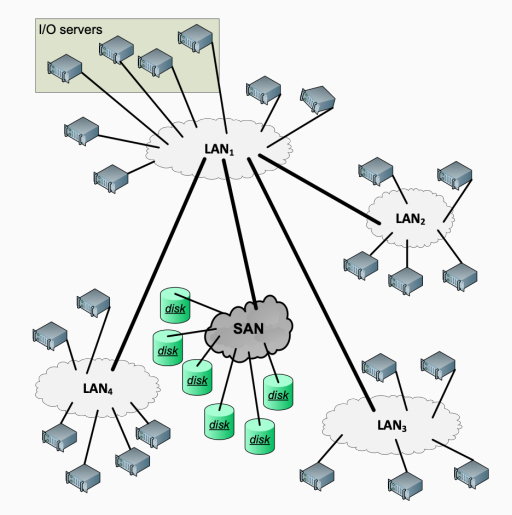
\includegraphics[scale=0.35]{images/GPFS.png}
    \caption{GPFS}
    \label{fig:gpfs}
\end{figure}

One important feature that GPFS introduced is a method of handling potential error: GPFS records all metadata updates in a log file that can be used to retrieve back information if errors on the file system occur.

One problem of the GPFS system is data striping that provides the segmentation of data. This policy improves performances (because it allow concurrent access) but since data are segmented and stored in different places, when the disk fails, a large number of files are affected.


\subsubsection{Google File System}
The \textbf{Google File System} (GFS) was developed in the late 90s.
Its design has the following features:
\begin{itemize}
    \item Scalability and reliability are critical. These aspects are because GFS uses thousands of storage systems to provides petabytes of storage to a large user community;
    \item The majority of file sizes range from few GB to hundreds of TB;
    \item Most common operations in the GFS are reading and appending something to existing files;
    \item Sequential read operation;
    \item Since file sizes are quite large, files are segmented in large chunks (that work with the TCP connection protocol).
    
    Chunks are fixed-size segments of 64 MB. They are quite large because:
    \begin{itemize}
        \item they work well with large files;
        \item they reduce the total metadata (less files means less metadata);
        \item multiple likelihood operations will be directed to the same chunk (so you can work inside the same chunk with less overhead; this means working with the same server);
    \end{itemize}
    Chunks are stored on Linux File System and are replicated on multiple sites.
    
    At the time of file creation each chunk is assigned a unique chunk handle. They are put in chunk servers (every chunk server is assigned to a set of chunks and uses a communication network to work with the master);
    \item GFS builds cluster around high-bandwidth (and it separates the control flow from data one); 
    \item Eliminates caching at the client site (leaving it only on the server side);
    \item Have a master that controls the entire cluster (it will maintain state information about all the system components) in order to "enter" the cluster", we have to communicate with it. The master node is the mechanism that allows consistency;
    \item GFS introduced checkpointing, recovering and a garbage collection system.
\end{itemize}

\begin{figure}[h!]
    \centering
    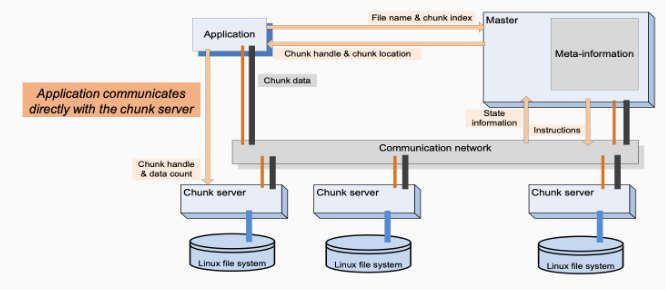
\includegraphics[scale=0.35]{images/GFS arch.png}
\end{figure}

Let's see how a write request is performed:
\begin{itemize}
    \item The client contacts the master which assigns a lease to one of the chunk servers; 
    \item The master replies with the ID of a primary and secondary chunk servers (that hold replicas of the chunk);
    \item The client sends data to all chunk servers that hold replicas (using the chunk handlers);
    \item Once it got an ack from all chunk server that hold replicas, the client send a write request to primary chunk server; 
    \item Primary chunk server sends the write request to all secondaries;
    \item Each secondary applies mutations in the order of the sequence number and sends ack back to primary;
    \item After receiving ack from all secondaries, primary sands an ack to the client.
\end{itemize}


\subsection{Locks and consensus}
Operating systems use lock managers to organise and serialise access to resources. In particular locks enable controlled access to shared storage and ensure atomicity of read and write operations (to avoid any collision).

Locks are allowed by the presence of a leader that is referred for getting information. It's elected through consensus. Election are implemented by a consensus protocol that accords everybody about a master.

To lock some resources we can use a distributed approach or a locking service (library to make process talk to each other asking for accesses).

The locks are discriminated for their effect:
\begin{itemize}
    \item \textbf{Advisory locks} are based on the assumption that all processes respects some rules (all file can have the access of the file);
    \item \textbf{Mandatory locks} block access to the locked objects to all processes that do not hold the locks;
\end{itemize}
and for the time:
\begin{itemize}
    \item \textbf{Fine-grained locks} can be held for only a very short time;
    \item \textbf{Coarse-grained locks} held the block for a longer time;
\end{itemize}


\subsubsection{Chubby}
Chubby is a very reliable and distributed lock service developed by Google for coarse-grained synchronization of distributed systems.
It's developed for a large number of machines connected by high-speed network and provides an interface much like a distributed file system.
It's an \textbf{advisory lock} and uses PAXOS\footnote{It's a family of protocols for solving consensus problems in a network} to ensure liveness.

The design of chubby it's not complicated and it consist of two main component that communicate via RPC (a replica server and a library).

Chubby cell consists of a small set of servers (typically 5) known as replicas that use PAXOS to elect a master and replicate logs. Read and write requests are satisfied by the master alone.
\begin{figure}[h!]
    \centering
    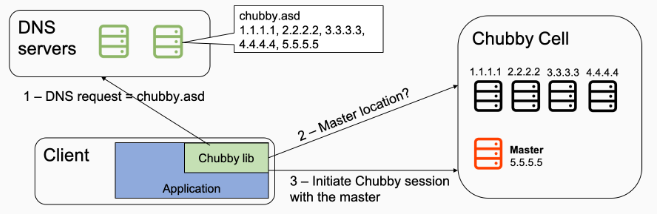
\includegraphics[scale=0.35]{images/chubbydesign.png}
\end{figure}

Chubby exports a file system interface, simpler than Unix, to provide some information. This file system interface is a tree of files and directories (with name components separated by /); each directory contains a list of child files and other sub-directories.
\begin{table}[h!]
    \centering
    \begin{tabular}{c c c}
          ls / & asd / & dunno/nothingJS\\
          is a prefix common & name of the & is the named chubby cell\\
          to all chubbys (lock service) & chubby cell 
    \end{tabular}
\end{table}

Chubby works with \textbf{nodes} that represent a file or directory. Each file can be either permanent or ephemeral and have some metadata and handlers associated to. In Chubby you can ask to open/close a node, to read/write contents and to  acquire/delete nodes.


\subsection{Distributed databases}
The \textbf{Google big table} (GBT) is a distributed storage system for managing structured data. 

Its design features are:
\begin{itemize}
    \item designed to scale to a very large size;
    \item not a relational database;
    \item designed as a key/value sorted and multi-dimensional map;
    \item flexible
    \item high performance solution
\end{itemize}

\begin{figure}[h!]
    \centering
    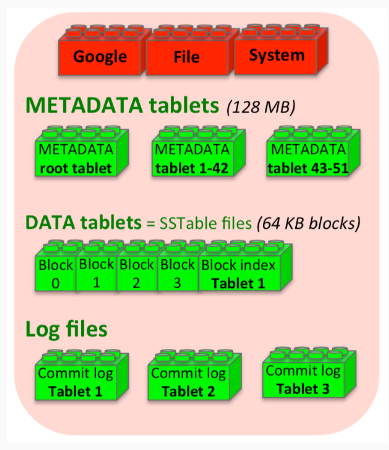
\includegraphics[scale=0.35]{images/GBTstruct.png}
\end{figure}

Being a sorted map, it has a set of columns associated with certain keys and a set of rows associated to entries (in form of strings of x bytes). Each cell is than a non interpreted array of bytes.

There's than a final dimension that's the timestamp with whom every information is recorded.

Rows are divided in groups of rows, called tablets.

The major components of GBT are:
\begin{itemize}
    \item One \textbf{Master} server that:
    \begin{itemize}
        \item assigns tablets to tablet servers;
        \item detects the addition and expiration of tablet server;
        \item balances tablet server load;
        \item does the Garbage collecting of files in GFS;
        \item handles schema changes.
        \item 
    \end{itemize}
    \item Many \textbf{Tablet} servers, each one:
    \begin{itemize}
        \item manages a set of tablets;
        \item handles read and write request to the tablets;
        \item splits tablets that have grown too large.
    \end{itemize}
    \item The \textbf{Client} that does not rely on the master (for tablet location and information) but instead communicates directly with tablet servers for reads and writes.
\end{itemize}

Each tablet is than assigned to one tablet server at time by the server (with a tablet load request to the server).
The tracking is realized by Chubby. So the Bigtable service works only if Chubby is available, otherwise it will be unavailable too.

When a tablet server starts, it creates and acquires an exclusive lock on a uniquely-named file in a specific Chubby directory.

Tablet server stops serving its tablets if it loses its exclusive Chubby lock. Master is responsible for detecting when a tablet server is no longer serving its tablets. To ensure that a Bigtable cluster is not vulnerable to networking issues if the master's Chubby session expires it will kills itself.

%QUESTA PARTE LA FINISCO DOMANI